\chapter{User Interface}

\section{Client}

The Kobold Client is based on Eclipse. Eclipse is a kind of universal tool 
platform - an open extensible IDE for anything and nothing in particular. Its 
user interface consists of views and editors. In editors you can both see and 
alter the data which is displayed whereas in views you can only look at the data 
but not alter it.

\subsection{Main Window}
In the Main Window you can see the following editors and views (see \ref{main}):
\begin{itemize}
	\item Architecture Editor
	\item Architecture Tree
	\item Navigator
	\item Workflow View
	\item Minimap
\end{itemize}

\begin{figure}[h!]
\begin{center}
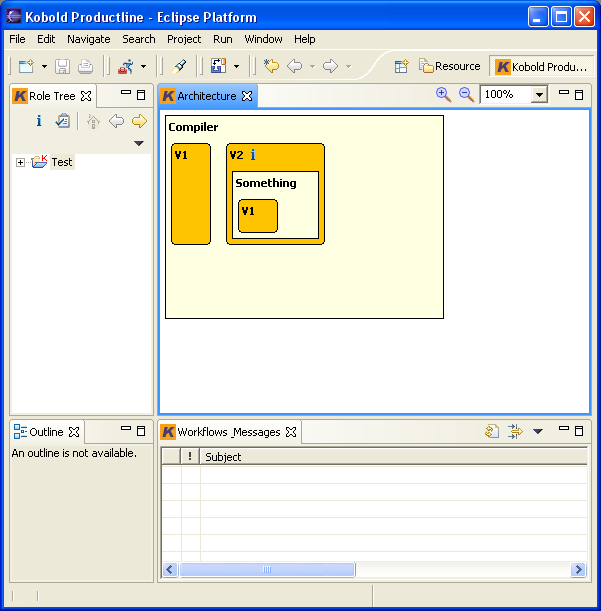
\includegraphics[width=17cm]{main.png}
   \caption{Main Window}
\label{main}
\end{center}
\end{figure}\par

The menu offers you in addition to the Eclipse standard options the following
possibilities:
\begin{itemize}
	\item Creating a new Kobold project
	\item Changing Kobold properties
\end{itemize}

\subsubsection{Creating a new project}

In the File menu select 'New' and then 'Kobold PLAM Project'. The Kobold wizard opens.
Enter the url of your Kobold server, your username and password. Then press
"test connection". If the test succeeds, the "next" button is enabled (see \ref{wizard1}).

\begin{figure}[h!]
\begin{center}
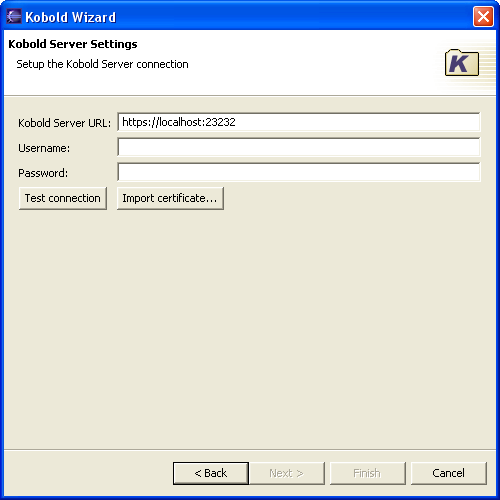
\includegraphics[width=10cm]{wizard1.png}
   \caption{Kobold wizard}
\label{wizard1}
\end{center}
\end{figure}\par

Before you proceed, you have the possibility to import a new certificate. In order to do this,
press the button 'import certificate...'. A new dialog opens (see \ref{certificate}) where you 
can enter an alias and your new certificate. Confirm with 'OK'.

\begin{figure}[h!]
\begin{center}
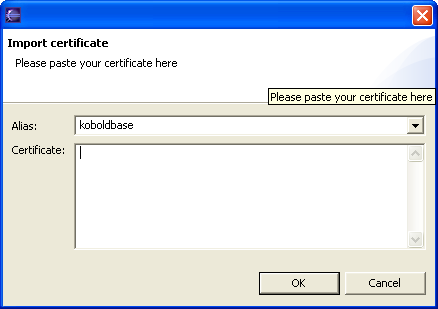
\includegraphics[width=10cm]{certificate.png}
   \caption{Importing a Certificate}
\label{certificate}
\end{center}
\end{figure}\par

After that you choose the productline you want to check out (see \ref{wizard2}).

\begin{figure}[h!]
\begin{center}

\includegraphics[width=10cm]{wizard2.png}
   \caption{Kobold wizard}
\label{wizard2}
\end{center}
\end{figure}\par

In the last step you have to enter the name of the project you want to create (see \ref{wizard3}).

\begin{figure}[h!]
\begin{center}
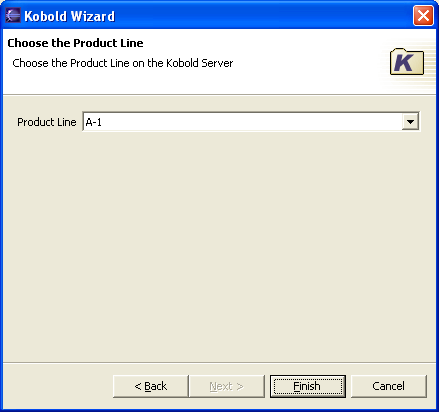
\includegraphics[width=10cm]{wizard3.png}
   \caption{Kobold wizard}
\label{wizard3}
\end{center}
\end{figure}\par

A new project has been created. You can open the different views and editors through the Window menu
and 'show view'. 

\subsubsection{Setting the Kobold preferences}
In the Kobold Client menu, select 'Window' and then 'Preferences'. The preferences
dialog opens (see \ref{pref}). Open the Kobold tree. In the SSL tab you can enter the 
properties for the Kobold Client. They resemble your SAT properties (see chapter '4.3 Server 
Administration Tool').
The VCM Configuration allows you to save your username, password and script for the
communication with the projects' repositories.

\begin{figure}[h!]
\begin{center}
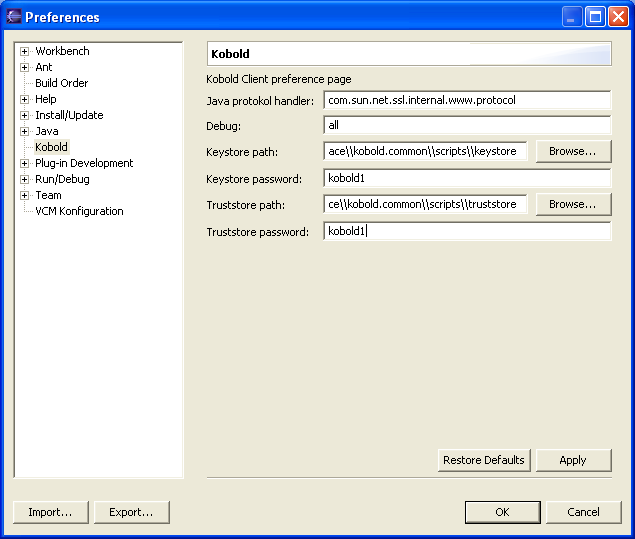
\includegraphics[width=17cm]{pref.png}
   \caption{Kobold preferences}
\label{pref}
\end{center}
\end{figure}\par



\subsection{Architecture Editor}

The Architecture Editor (see \ref{architecture}) displays the architecture of the product,
or productline respectively, that is selected in the Architecture Tree. \par

\begin{figure}[h!]
\begin{center}

\includegraphics[width=15cm]{architecture.png}
   \caption{Architecture Editor}
\label{architecture}
\end{center}
\end{figure}\par

Architectures are directed graphs that consist of nodes and edges. 
Nodes represent components, variants and releases. Directed edges represent
any relationship between nodes.\par

The Architecture Editor offers you the following options:
\begin{itemize}
	\item Create a core asset/component
	\item Configure a core asset/component
	\item Createa variant
	\item Configure a variant
	\item Create a release
	\item Configure a release
	\item Delete a core asset/component, variant or release
	\item Create a meta node
	\item Delete a meta node
	\item Create a dependency edge
	\item Create an exclusion edge
	\item Delete an edge
	\item Mark a product, component, variant or release "deprecated"
	\item Set the maintainers of a productline, product or component
	\item Move an item
	\item Change the size of an item
	\item Compose a product
	\item Configure a product
	\item Edit the repository descriptor of a product
	\item Export
\end{itemize}

Most of the options can be reached through the palette (see \ref{palette}).
You can find it to the right of the Architecture Editor. If offers you the tools
to work with the Architecture Editor and opens up when you click on it.

\begin{figure}[h!]
\begin{center}

\includegraphics[width=4cm]{palette.png}
   \caption{The palette}
\label{palette}
\end{center}
\end{figure}\par


\subsubsection{Creating a Core Asset/component}

In the pallete select the "component" item. Click within a variant or top-level in 
the Architecture Editor. A component is inserted (see \ref{component}) and a dialog opens where you can enter the meta data of
the component. By clicking on the border and pulling it you can simply change the size of the component. \par
Note: Core Assets/Components can only be inserted top-level or into variants.

\begin{figure}[h!]
\begin{center}

\includegraphics[width=6cm]{component.png}
   \caption{Component}
\label{component}
\end{center}
\end{figure}\par

\subsubsection{Configuring a core asset/component}
In the Architecture Editor right-click on the core asset/component you want to configure. 
A context menu opens where you choose 'Configure...'. This opens the Asset Configuration Dialog
for components (see \ref{configcomp}). Here you can change the name, description, maintainers and scripts for the
asset. You can also set the asset on deprecated if you like.

\begin{figure}[h!]
\begin{center}
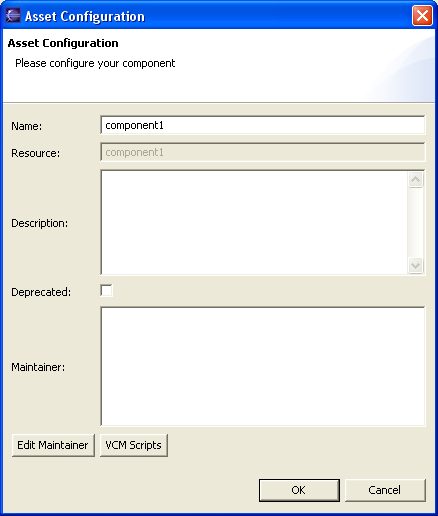
\includegraphics[width=12cm]{configcomp.png}
   \caption{Asset Configuration Dialog for Components}
\label{configcomp}
\end{center}
\end{figure}\par

\subsubsection{Creating a variant}

In the pallete select the "variant" item. Click within a component in 
the Architecture Editor. A variant is inserted (see \ref{variant}) and a dialog opens where you can enter the meta data of
the variant. By clicking on the border and pulling it you can simply change the size of the variant. \par
Note: Variants can only be inserted into components.

\begin{figure}[h!]
\begin{center}

\includegraphics[width=10cm]{variant.png}
   \caption{Variant}
\label{variant}
\end{center}
\end{figure}\par


\subsubsection{Configuring a variant}
In the Architecture Editor right-click on the variant you want to configure. 
A context menu opens where you choose 'Configure...'. This opens the Asset Configuration Dialog
for variants (see \ref{configvar}). Here you can change the name, description and scripts for the
asset. You can also set the asset on deprecated if you like.

\begin{figure}[h!]
\begin{center}
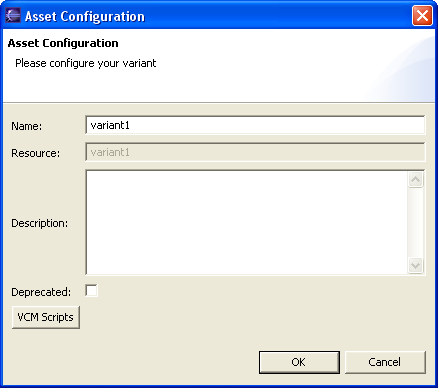
\includegraphics[width=12cm]{configvar.png}
   \caption{Asset Configuration Dialog for Variants}
\label{configvar}
\end{center}
\end{figure}\par

\subsubsection{Creating a release}

In the pallete select the "release" item. Click within a variant in 
the Architecture Editor. A release is inserted (see \ref{release}) and a dialog opens where you can enter the data of
the release. For each file of the surrounding variant you can select the revision number you want to add to the release. 
By clicking on the border and pulling it you can simply change the size of the release. \par
Note: Releases can only be inserted into variants.

\begin{figure}[h!]
\begin{center}

\includegraphics[width=10cm]{release.png}
   \caption{Release}
\label{release}
\end{center}
\end{figure}\par


\subsubsection{Configuring a release}
In the Architecture Editor right-click on the release you want to configure. 
A context menu opens where you choose 'Configure...'. This opens the Asset Configuration Dialog
for releases (see \ref{configrel}). Here you can change the name, description, resources and scripts for the
asset. You can also set the asset on deprecated or mark it as a release if you like.

\begin{figure}[h!]
\begin{center}
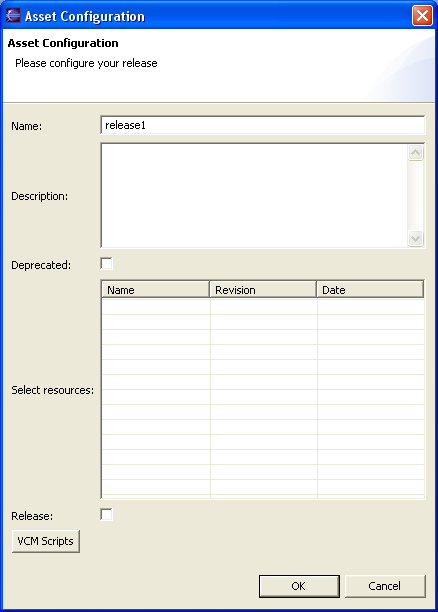
\includegraphics[width=12cm]{configrel.png}
   \caption{Asset Configuration Dialog for Releases}
\label{configrel}
\end{center}
\end{figure}\par


\subsubsection{Deleting a core asset/component, variant or release}

Right-click on the item you want to delete and choose "delete" in the context
menu. Alternatively you
can select the item and press "Del" on your keyboard. Is the item used in other projects
you will be notified and be able to cancel the deletion process.


\subsubsection{Creating a meta node}

In the pallete select the "meta node" item. Click within the Architecture Editor. 
A meta node is inserted (see \ref{meta}). Possible meta node types are AND and OR. Be careful with
the direction of the edges that are linked to a meta node! In the following architecture component A
needs components B and C. But components B and C are independent of component A (see \ref{example}).

\begin{figure}[h!]
\begin{center}

\includegraphics[width=4cm]{metanode.png}
   \caption{Some meta nodes}
\label{meta}
\end{center}
\end{figure}\par

\begin{figure}[h!]
\begin{center}

\includegraphics[width=10cm]{example.png}
   \caption{Meta node example}
\label{example}
\end{center}
\end{figure}\par

\subsubsection{Deleting a meta node}

Right-click on the meta node you want to delete and choose "delete" in the context
menu. Alternatively you
can select the node and press "Del" on your keyboard.

\subsubsection{Marking a product, component, variant or release as "deprecated"}
Right-click on the object and choose "configure". The Asset Configuration dialog (see \ref{configp}, \ref{configcomp}, \ref{configvar} and \ref{configrel}) opens where you can
mark the check-box 'deprecated'. This sets the object on deprecated. Deprecated objects are grey with a 
red cross in the upper right-hand corner (see \ref{deprecated}).

\begin{figure}[h!]
\begin{center}

\includegraphics[width=7cm]{deprecated.png}
   \caption{Deprecated component}
\label{deprecated}
\end{center}
\end{figure}\par



\subsubsection{Creating a dependency edge}

In the pallete select the "include edge" item. Select an item in the Architecture Editor
as the starting point. The next item you select will be the aiming point (see \ref{include}).

\begin{figure}[h!]
\begin{center}

\includegraphics[width=10cm]{include.png}
   \caption{Dependency edge}
\label{include}
\end{center}
\end{figure}\par

\subsubsection{Creating an exclusion edge}

In the pallete select the "exclude edge" item. Select an item in the Architecture Editor
as the starting point. The next item you select will be the aiming point (see \ref{exclude}).

\begin{figure}[h!]
\begin{center}

\includegraphics[width=10cm]{exclude.png}
   \caption{Exclusion edge}
\label{exclude}
\end{center}
\end{figure}\par

\subsubsection{Deleting an edge}

Right-click on the edge you want to delete and choose "delete" in the context menu.
Alternatively you can select the edge and press "Del" on your keyboard.


\subsubsection{Setting the maintainers of a productline, product or component}
Right-click on the component or name of the product(line) and choose "configure". The Asset Configuration dialog (see \ref{configcomp}, \ref{configp} and \ref{configpl}) opens.
Press the 'Edit Maintainer' button. A new window opens where you can select the users you want to make maintainers of
the product(line)/component (see \ref{maintainer}). After pressing 'OK' you can see the new maintainers in the Asset Configuration
dialog.

\begin{figure}[h!]
\begin{center}
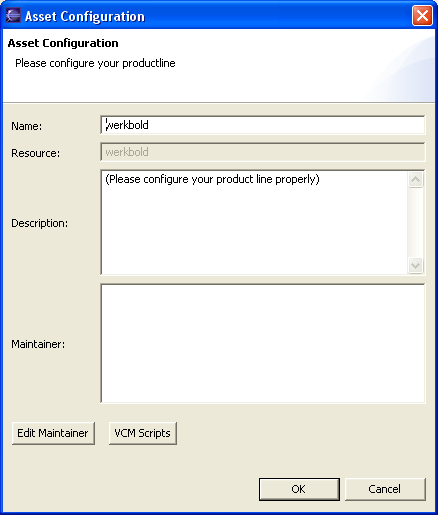
\includegraphics[width=12cm]{configpl.png}
   \caption{Asset Configuration Dialog for Productlines}
\label{configpl}
\end{center}
\end{figure}\par

\begin{figure}[h!]
\begin{center}
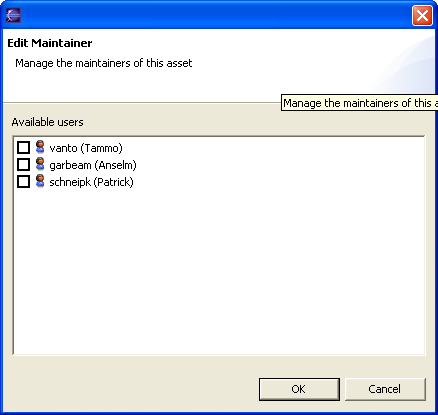
\includegraphics[width=10cm]{maintainer.png}
   \caption{Selecting maintainers}
\label{maintainer}
\end{center}
\end{figure}\par


\subsubsection{Moving an item}
You can move any item by clicking on the item and pulling it.

\subsubsection{Changing the size of an item}
You can change the size of an item by clicking on the border of the item and pulling it.


\subsubsection{Composing a product}

In the palette press 'compose product'. The components, etc. in the architecture editor turn
grey. You can now select the components, variants and releases you want to include into
you new product. The chosen objects turn blue (see \ref{compose}). When done press the 
'create product' button in the Architecture Editor. A dialog opens where you can enter
the name, resource, description, maintainers, scripts and repository descriptor of your new product. After confirming the dialog, you can see
your new product in the Architecture Tree and Architecture Editor.

\begin{figure}[h!]
\begin{center}

\includegraphics[width=12cm]{composeproduct.png}
   \caption{Composing a Product}
\label{compose}
\end{center}
\end{figure}\par

\subsubsection{Configuring a product}
In the Architecture Editor right-click on the product you want to configure. 
A context menu opens where you choose 'Configure...'. This opens the Asset Configuration Dialog
for products (see \ref{configp}). Here you can change the name, resource, description, maintainers, repository descriptor and scripts for the
asset. You can also set the asset on deprecated if you like.

\begin{figure}[h!]
\begin{center}
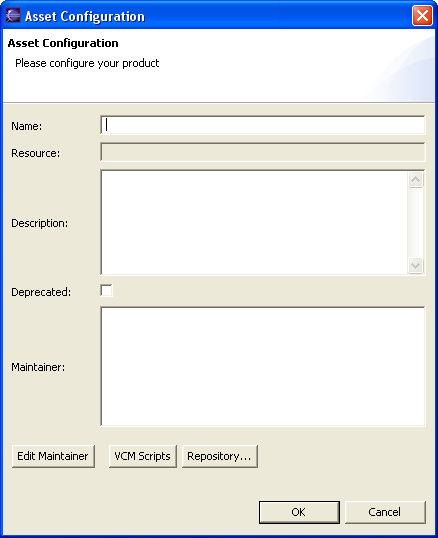
\includegraphics[width=12cm]{configp.png}
   \caption{Asset Configuration Dialog for Products}
\label{configp}
\end{center}
\end{figure}\par


\subsubsection{Editing the repository descriptor of a product}
In the Architecture Editor right-click on the product. A context menu opens where
you choose 'Configure Asset'. This opens the Asset Configuration dialog for
products (see \ref{configp}). Press the 'Repository...' button and a new dialog opens (see \ref{repository}).
Here you can change the data of the repository that saves the data of the product. Confirm with 'OK'.

\begin{figure}[h!]
\begin{center}
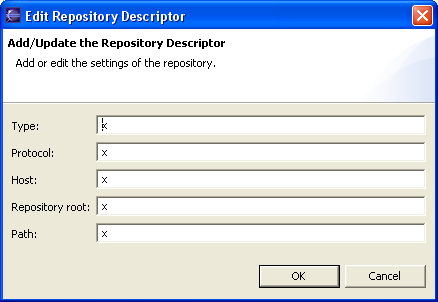
\includegraphics[width=12cm]{repository.png}
   \caption{Edit Repository Descriptor}
\label{repository}
\end{center}
\end{figure}\par



\subsubsection{Export}

Select the productline, product, component or variant you want to export. In the
context menu of the object select "export" (see \ref{archcontext}). A wizard opens (see \ref{export}) where you can enter
the path and name of the gxl-file. Alternatively you can enter 
the data through the "browse" dialog. To start the export, press the OK button.
You are able to see the status of your export in the wizard which will close after
the export is finished. If you decide not to do the export, simply press the 
"cancel" button.

\begin{figure}[h!]
\begin{center}

\includegraphics[width=10cm]{architecturekontext.png}
   \caption{Context menu of the Architecture View}
\label{archcontext}
\end{center}
\end{figure}\par

\begin{figure}[h!]
\begin{center}
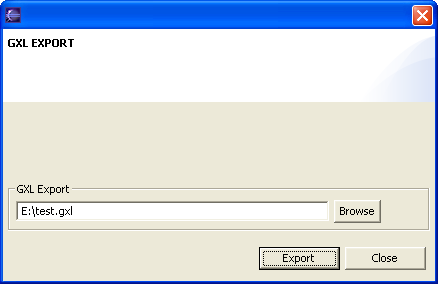
\includegraphics[width=10cm]{export.png}
   \caption{Export wizard}
\label{export}
\end{center}
\end{figure}\par







\subsection{Architecture Tree}

The Architecture Tree shows the current projects that are checked out in your workspace 
(see \ref{roletree}).
A project is always a productline. You can navigate between the 
different projects by selecting them. If you open the tree, you see the name
of the productline. Double-click on 'Architecture' and the Architecture Editor will open. The open tree also 
displays all products, PLEs and core assets that belong to the productline.

\begin{figure}[h!]
\begin{center}

\includegraphics[width=7cm]{roletree.png}
   \caption{Architecture Tree}
\label{roletree}
\end{center}
\end{figure}\par

When you right-click on a project, a context menu will open where you can choose 
between different actions (see \ref{rolekontext} and \ref{rolekontext2}). The possible actions are different
depending on which asset you open the context menu on. Possible actions are:

\begin{itemize}
	\item Create a new user
	\item Change password
	\item Update full name
	\item Configure asset
	\item Suggest an asset for a Core Group
	\item Generate AssetInfo document
	\item Export
	\item Import
	\item Add to Product
	\item Delete Asset
	\item Version Control
\end{itemize}

\begin{figure}[h!]
\begin{center}

\includegraphics[width=8cm]{rolekontext.png}
   \caption{Architecture Tree Context Menu 1}
\label{rolekontext}
\end{center}
\end{figure}\par

\begin{figure}[h!]
\begin{center}

\includegraphics[width=8cm]{rolekontext2.png}
   \caption{Architecture Tree Context Menu 2}
\label{rolekontext2}
\end{center}
\end{figure}\par


\subsubsection{Creating a user}

Right-click in the architecture tree. In the context menu choose
'create new user'. The User Manager (see \ref{createuser1}) opens where you see a list of all existing users.
In order to create a new user, enter the username, name and password of the new user and press the 'add user' button.
You
can see the new user in the list of the User Manager.

\begin{figure}[h!]
\begin{center}
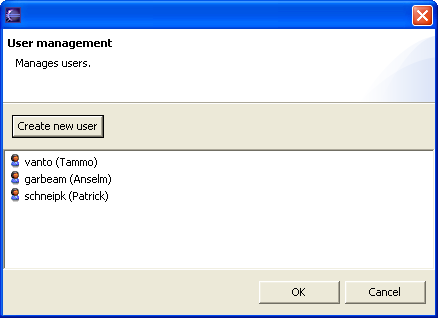
\includegraphics[width=10cm]{createuser1.png}
   \caption{Create a new user}
\label{createuser1}
\end{center}
\end{figure}\par


\subsubsection{Changing your password}

Right-click in the architecture tree and select 'update password'. A dialog opens where you can
enter your new password (see \ref{password}). Confirm the password and press 'OK'. Your password has been changed.

\begin{figure}[h!]
\begin{center}
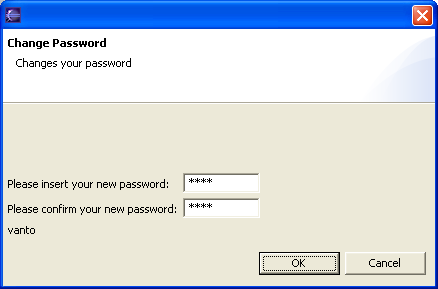
\includegraphics[width=10cm]{password.png}
   \caption{Change your password}
\label{password}
\end{center}
\end{figure}\par

\subsubsection{Updating your full name}
Right-click in the architecture tree and select 'update full name'. A dialog opens where you can
enter your new full name (see \ref{fullname}). Confirm the changes with your password and press 'OK'. Your full name has been changed.

\begin{figure}[h!]
\begin{center}
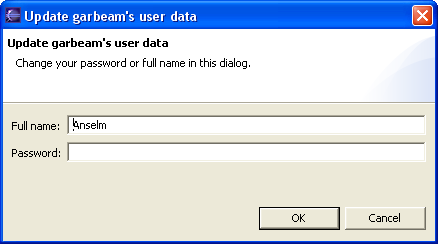
\includegraphics[width=10cm]{updatefullname.png}
   \caption{Update your full name}
\label{fullname}
\end{center}
\end{figure}\par

\subsubsection{Configure Asset}
In the architecture tree right click on the asset you want to configure and select
'configure asset...'. The corresponding dialog will open. For more information see
'Architecture Editor'.

\subsubsection{Suggesting an asset for a Core Group}

In the Architecture Tree, select the asset you want to suggest and right-click on it. The context menu opens where
 you choose the option 'Suggest asset for core group'. A dialog opens where
 you can select the type of recipient, that is whether the suggestion is to be sent to a PE or a PLE. After
 that decision a Workflow
window opens where you can enter the name of the asset and the username of the
PE/PLE you want to send the message to. You can also enter an additional comment you want 
the PE/PLE to read. Send the message by pressing the "Transmit" 
button. Pressing the "Cancel" button will close the window without sending 
your message (see \ref{core1}).

\begin{figure}[h!]
\begin{center}
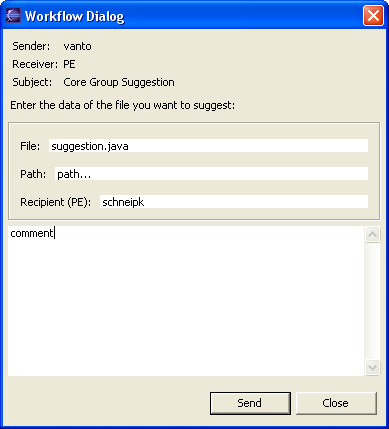
\includegraphics[width=12cm]{core1.png}
   \caption{Suggesting an asset for a Core Group}
\label{core1}
\end{center}
\end{figure}\par


\subsubsection{Generating an AssetInfo document}
In the architecture tree right-click on the object (productline, product, component, variant, release) you want the document about
and select 'generate AssetInfo document...'. A 'Save as' dialog opens where you can select the parent folder into which the pdf-file
will be saved. Confirm by pressing the 'OK' button and the pdf-file is created.

\subsubsection{Export}
In the architecture tree right-click on the asset you want to export and select
'GXL Export'. The corresponding dialog will open. For more information see
'Architecture Editor'.

\subsubsection{Import}
In the architecture tree right-click on a product and choose 'GXL Import...'. A dialog
opens (see \ref{import}) where you can enter the name and path of the gxl-file you want to import. Click 
'proceed' to finish.

\begin{figure}[h!]
\begin{center}
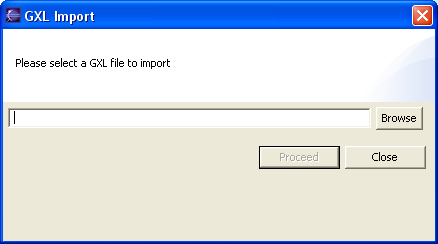
\includegraphics[width=10cm]{import.png}
   \caption{Import}
\label{import}
\end{center}
\end{figure}\par



\subsubsection{Add Asset to Product}
In the architecture tree right-click on the variant you want to add to a product
and choose 'Add to Product'. A dialog opens where you can choose the products you
want to add the variant to (see \ref{addproduct}). When done confirm by pressing
'OK'. The variant is added to the chosen products.


\begin{figure}[h!]
\begin{center}
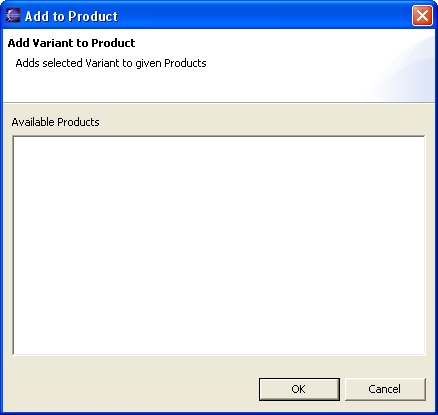
\includegraphics[width=10cm]{addtoproduct.png}
   \caption{Add an Asset to a Product}
\label{addproduct}
\end{center}
\end{figure}\par


\subsubsection{Delete Asset}
In the architecture tree right-click on the asset you want to delete and choose
'delete asset'. A dialog opens (see \ref{delete}) which asks you if you really want to delete the asset.
If you press 'yes', the asset will be deleted. If you press 'no', the asset and its
subassets will
be marked as deprecated. You can change this status anytime through the asset 
configuration dialog. 


\begin{figure}[h!]
\begin{center}
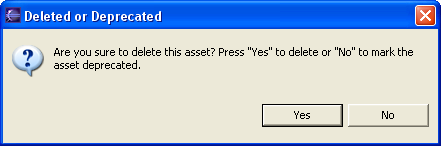
\includegraphics[width=10cm]{deleteasset.png}
   \caption{Deleting an Asset}
\label{delete}
\end{center}
\end{figure}\par

\subsubsection{Version Control}
Right-click on an asset and choose 'Version Control'. Another menu opens where you can choose
between different version control actions (see \ref{vcm}). Among those are:
\begin{itemize}
	\item Checkout
	\item Import
	\item Add
	\item Update
	\item Commit
\end{itemize}

\begin{figure}[h!]
\begin{center}

\includegraphics[width=10cm]{vcm.png}
   \caption{Version Control Actions}
\label{vcm}
\end{center}
\end{figure}\par





\subsection{Navigator}
The Navigator hides behind the Architecture Tree and is brought to the front by
clicking on it (see \ref{navigator}).

\begin{figure}[h!]
\begin{center}

\includegraphics[width=10cm]{roletree2.png}
   \caption{Navigator}
\label{navigator}
\end{center}
\end{figure}\par

It shows the folders the way they are saved on your hard disk and in the repositories.
Here you can use the normal Eclipse actions you can easily look up in the Eclipse help.






\subsection{Workflow View}

In the bottom of the window you can see the Workflow View which displays all 
the messages and workflows for the current user (see \ref{workflow}). 

\begin{figure}[h!]
\begin{center}

\includegraphics[width=15cm]{workflow.png}
   \caption{Workflow/Task View}
\label{workflow}
\end{center}
\end{figure}\par

The icon in front of each message/workflow helps you to determine whether the entry is a 
workflow or a message. A 'W' represents a workflow, a 'K' represents a Kobold message.\par

Double-click on an entry and a 
separate dialog will be opened where you can read the details of that message or
workflow (see \ref{workflowdialog}).

\begin{figure}[h!]
\begin{center}
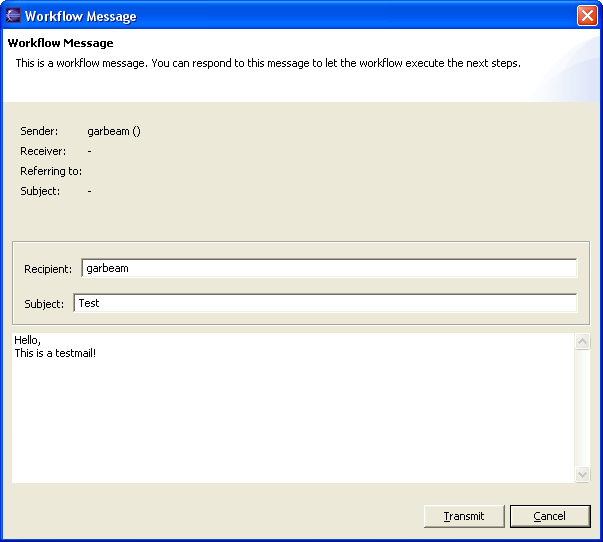
\includegraphics[width=5cm]{writemail.png}
   \caption{Message Dialog}
\label{workflowdialog}
\end{center}
\end{figure}\par

When you right-click on a message, a context menu will open where you can choose 
between different actions (see \ref{workflowkontext}). Among these are:

\begin{itemize}
	\item Fetching messages
	\item Deleting the selected message
\end{itemize}

\begin{figure}[h!]
\begin{center}

\includegraphics[width=7cm]{workflowkontext.png}
   \caption{Message Context Menu}
\label{workflowkontext}
\end{center}
\end{figure}\par

The Workflow View offers you the following additional options:
\begin{itemize}
	\item Writing a mail
	\item Answering a mail
	\item Suggesting an asset for a Core Group
	\item Dealing with a Core Group suggestion
\end{itemize}


\subsubsection {Fetching messages}

Select a project. Right-click in the Workflow View or open the corresponding menu. Choose "Fetch message".
Your new messages are being fetched and displayed in the Workflow View.


\subsubsection{Deleting a message}

Right-click on the message and choose "Delete message" in the context menu.


\subsubsection{Writing a mail}

In the menu of the Workflow View select "new mail". A Workflow window opens where
you can enter your message, the subject and the recipient of the message. Send the
message by pressing the "Transmit" button. Pressing the "Cancel" button will close the window
without sending your message (see \ref{writemail}).

\begin{figure}[h!]
\begin{center}
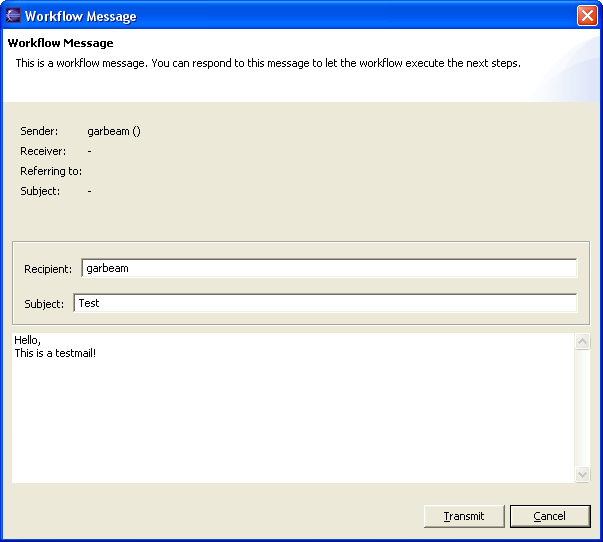
\includegraphics[width=10cm]{writemail.png}
   \caption{Write a new mail}
\label{writemail}
\end{center}
\end{figure}\par

\subsubsection{Answering a mail}

In the Workflow View double-click on the mail you want to answer. A Workflow
window opens where you can see the message text of the mail. Below you can enter
the subject and the text of your reply. Send the answer by pressing the "Transmit" 
button. Pressing the "Cancel" button will close the window without sending 
your message (see \ref{answermail}).

\begin{figure}[h!]
\begin{center}
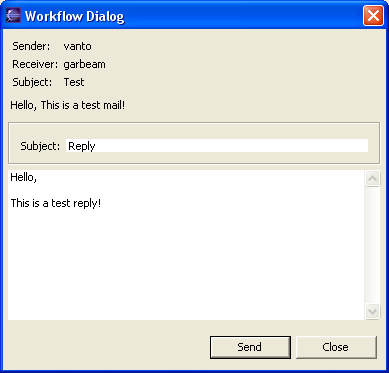
\includegraphics[width=10cm]{answermail.png}
   \caption{Answer a mail}
\label{answermail}
\end{center}
\end{figure}\par

\subsubsection{Suggesting an asset for a Core Group}

In the menu of the Workflow View select 'Suggest asset for core group'. A dialog opens where
 you can select the type of recipient, that is whether the suggestion is to be sent to a PE or a PLE. After
 that decision a Workflow
window opens where you can enter the name of the asset and the username of the
PE/PLE you want to send the message to. You can also enter an additional comment you want 
the PE/PLE to read. Send the message by pressing the "Transmit" 
button. Pressing the "Cancel" button will close the window without sending 
your message (see \ref{core1}).


\begin{figure}[h!]
\begin{center}
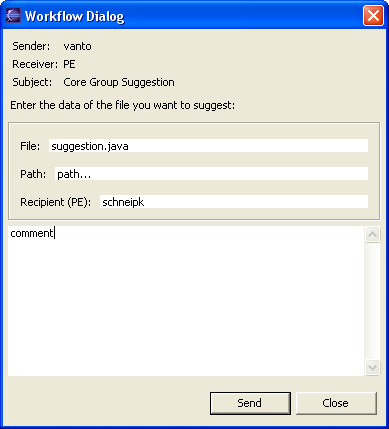
\includegraphics[width=10cm]{core1.png}
   \caption{Suggesting a file for a Core Group}
\label{core1}
\end{center}
\end{figure}\par

\subsubsection{Dealing with a Core Group suggestion}

In the Workflow View double-click on the Core Group suggestion message. A Workflow
window opens where you can see the message of the programmer (see \ref{core2}) or PE (see \ref{core3}). Below you
can select whether you agree to the suggestion or whether you decline it. You can also
enter an additional comment if you like. Send the message by pressing the "Transmit" 
button. Pressing the "Cancel" button will close the window without sending 
your message.\par
Note: The file will not be automatically uploaded and committed. The PLE has to do
this manually.

\begin{figure}[h!]
\begin{center}
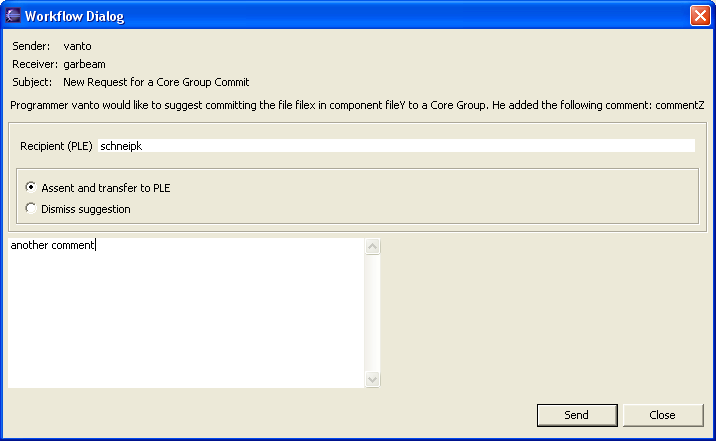
\includegraphics[width=14cm]{core2.png}
   \caption{Dealing with a Core Group suggestion - PE}
\label{core2}
\end{center}
\end{figure}\par

\begin{figure}[h!]
\begin{center}
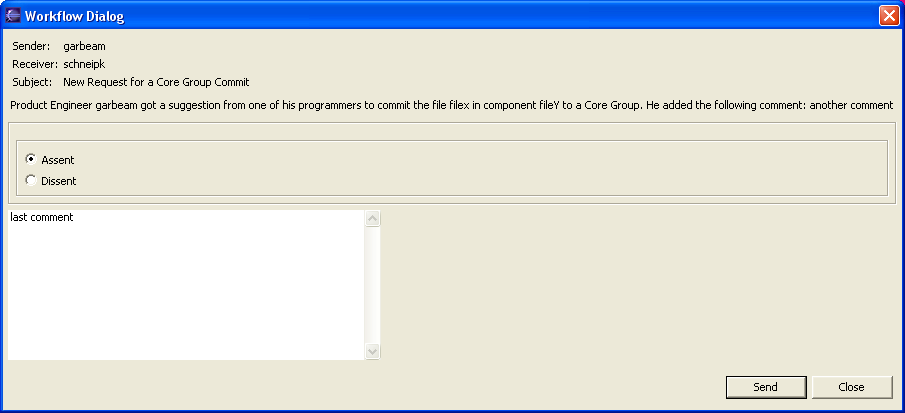
\includegraphics[width=14cm]{core3.png}
   \caption{Dealing with a Core Group suggestion - PLE}
\label{core3}
\end{center}
\end{figure}\par


\subsection{Minimap}

The Minimap (see \ref{map}) is on the left side beneath the Architecture Tree. It shows the whole architecture.
By clicking at one spot on the map, the Architecture Editor automatically centers on that
spot. You can also click on the coloured rectangle and pull it to another position. 
By doing this you can easily navigate through your architecture.

\begin{figure}[h!]
\begin{center}

\includegraphics[width=10cm]{outline.png}
   \caption{Minimap}
\label{map}
\end{center}
\end{figure}\par




\section{Server}

The Server administrates the data of each user and their responsibilities. Also it
offers the Clients a central message service . If a message is sent from a Client
to the Server, the Server checks the message for possible consequences which are
assigned to other clients as workflows. Besides the Server administrates the paths
and the access configurations of the repositories which save the data of the products
and the productlines.

\subsection{Changing the Server Properties}
When installing the server properties are automatically set for you. However, this section is for those
of you who want to change your server properties manually:

Edit the server.properties
file from {\it kobold.server/server.properties} to suite your local
requirements. Under UNIX this file might look similiar to the following
bits:

\begin{verbatim}
# Note storePath is the prefix path for all kobold stores!
kobold.server.storePath=[your storage path]
kobold.server.productStore=product.xml
kobold.server.userStore=user.xml
kobold.server.ruleset={path to ruleset]
#
java.protocol.handler.pkgs=com.sun.net.ssl.internal.www.protocol
javax.net.debug=none#all
javax.net.ssl.keyStore=[your keystore path]
javax.net.ssl.keyStorePassword=[your keystore passphrase]
javax.net.ssl.trustStore=[your truststore path]
javax.net.ssl.trustStorePassword=[your truststore passphrase]
\end{verbatim}

Under Windows-based systems you've to change the paths into a
DOS-alike format.

In the following table all properties are described in detail:

\begin{tabular}{|l|l|l|}\hline
\textbf{Property} &  \textbf{Description}\\ \hline
kobold.server.storePath  & destination path for files stored by the server \\ \hline
kobold.server.productStore & file name to store products and
productlines \\ \hline
kobold.server.userStore & file name to store user data \\ \hline
kobold.server.ruleset & path to your ruleset file \\ \hline
java.protocol.handler.pkgs & default protocol to commincate \\ \hline
javax.net.debug & debug level of net communication \\ \hline
javax.net.ssl.keyStore & path to your SSL keystore \\ \hline
javax.net.ssl.keyStorePassword & password to access your SSL keystore \\
    \hline
javax.net.ssl.trustStore & path to your SSL truststore \\ \hline
javax.net.ssl.trustStorePassword & password to access your SSL
truststore \\ \hline
\end{tabular}



\subsection{Creating a Workflow}

Workflows are triggered by specific rules which you can find in the ruleset.drl file.
Here you can find some existing rules as examples. \par

A rule consists of the following parts:
\begin{itemize}
	\item name
	\item parameters
	\item conditions
	\item one consequence
\end{itemize}
Rules are a mixture of XML and Java.\par

This is what a sample rule looks like: \\

$<$rule name = "Name of the rule"$>$\\
\begin{quote}
$<$parameter identifier = "spy"$>$\\
\begin{quote}
$<$java:class$>$ kobold.common.data.RPCSpy $<$/java:class$>$\\
\end{quote}
$<$/parameter$>$\par
$<$java:condition$>$ spy.getMethodName().equals("addUser") $<$/java:condition$>$\par
$<$java:consequence$>$ System.out.println("Rule fired."); $<$/java:consequence$>$\\
\end{quote}
$<$/rule$>$\par


The rule will only be fired when its conditions are true. If there are several conditions,
all of them have to be true. Conditions and consequence are written in Java.\par

For your own rules, the rule's parameter will always be an RPCSpy object of the package
kobold.common.data. Such an object is created whenever an action is being executed by the server.
These are in detail (using their actual method names):
\begin{itemize}
	\item addUser
	\item getAllUsers
	\item removeUser
	\item updateUserPassword
	\item updateUserFullName
	\item getProductlineNames
	\item getProductline
	\item updateProductline
	\item updateProduct
	\item updateComponent
\end{itemize}
The parameter RPCSpy will contain the methodName which you can get with the "getMethodName()" method. 
This returns one of the above Strings. An RPCSpy object also contains a vector of
arguments that were transmitted to the server for the execution. You have access to this vector through
the "getArguments()" method. \par
The ruleset.drl file contains sample rules for all actions.\par
In the last chapter you find the source code of the classes you need to work with for writing your own rules.






\section{Server Administration Tool (SAT)}

Kobold servers do not have to be administrated directly. Instead the Kobold System 
provides a stand-alone client with the sole purpose of administrating Kobold servers 
over a secure ssl-connection. \par

After having set the server's url and its administration password you have the following 
possibilities:

\begin{itemize}
	\item create a productline
	\item delete a productline
	\item create a new user
	\item remove a user
	\item assign an existing user to a productline as PLE
	\item remove a user's PLE rights for a productline
	\item get a list of all productlines
	\item get a list of all PLEs of a productline
	\item get a list of all users
\end{itemize}




\subsection{Setting up the server connection}
At startup the SAT tries per default to establish a connection to a server running 
at 'localhost' on port 23232 without a set administration password. You can change
those default settings at any time by entering the command 'setserver'.\par

After entering that command the current properties of the server connection are 
listed (note that the password is not shown in plain text). Enter '1' to change
the server's ip, '2' to change the server's port and '3' to change the administration
password.\par

If you decide to set or change a password the SAT provides secure password masking by
prompting a region of 8 randomly changing characters into which your input is - randomly - 
echoed to. This happens because it is not possible to prevent the java input stream from
echoing to the console. Nonetheless echoing into that region makes it virtually impossible 
to determine which of the prompted characters are echoed and which are generated randomly.\par

When you have finished modifiying the connection properties confirm by entereing 'p'. The SAT 
tries to establish the new connection. Enter 'c' to cancel the action.

\subsection{Creating a productline}
Enter the command 'newpl'. A listing is shown with the properties of the lately created
productline. You can change the properties as described above. By entering 'p' the SAT
tries to create a new productline with the current settings. \par

Please note that every productline of a Kobold server must have an unique name. Creation
of a productline with an already assigned name will be refused by the server.

\subsection{Deleting a product line}
Enter the command 'rempl'. All registered productlines' names are listed and you are 
asked to enter the name of the productline you want to remove. Once you have confirmed your 
entry, the productline is deleted.

\subsection{Assigning an existing user to a productline as PLE}
Enter the command 'assignple'. You are asked to enter the name of the person you want
to become PLE. Finally, enter the name of the productline you want to assign the new 
PLE to. Once you confirmed your entry, the user has PLE rights.

\subsection{Removing PLE rights}
Enter the command 'unassignple'. You are asked to enter the name of the user who shall 
no longer have PLE rights. Also, enter the name of the productline you want to
remove the PLE from. Once you confirmed your entry, the user is no longer PLE of
the entered product line.

\subsection{Getting a list of all existing commands}
Enter the command 'help' to get a list of all the commands of this tool and
their meanings.

\subsection{Getting information about SAT's version and licence}
Enter the command 'about' and you get information about the programm's version and licence.

\subsection{Creating a new user}
Enter the command 'newuser'. A listing is shown with the properties of the lately created
user, his/her username, fullname and initial password. After enetering 'p' a new user with
the shown properties is created on the server.\par

Note that every registered user needs to have its own unique username. Creation of a new user 
with a username that's already been registered will be refused by the server.

\subsection{Deleting a user}
Enter the command 'remuser'. A listing with all registered usernames is shown and you are
asked to enter the username of the user you like to remove from the server. A check is
performed to determine if the specified user is still assigned to an asset. If so, you are
informed by the SAT and given the possibility to cancel the action.

\subsection{Getting a list of all productlines}
Enter the command 'pllist' in order to get a list of all productlines registered on the 
current server.

\subsection{Getting a list of all ples of a productline}
Enter the command 'plelist' and then the name of the productline in order to get a list
 of the assigned ples.
 
\subsection{Getting a list of all registered users}
Enter the command 'userlist' in order to get a list of all registered users.

\subsection{Exiting the tool}
Enter the command "exit".






\subsection{Changing the SAT Properties}
When installing the SAT properties are automatically set for you. However, this section is for those
of you who want to change your SAT properties manually:

Edit the SAT.properties
file from {\it kobold.client.serveradmin/sat.properties} to suite your local
requirements. Under UNIX this file might look similiar to the following
bits:

\begin{verbatim}
#used to communicate with Kobold servers via ssl
java.protocol.handler.pkgs=com.sun.net.ssl.internal.www.protocol
javax.net.debug=none #all
javax.net.ssl.keyStore=/home/stsopra/werkbold/contan/workspace/kobold.common/kobold.common/scripts/keystore
javax.net.ssl.keyStorePassword=kobold1
javax.net.ssl.trustStore=/home/stsopra/werkbold/contan/workspace/kobold.common/kobold.common/scripts/truststore
javax.net.ssl.trustStorePassword=kobold1
\end{verbatim}

Under Windows-based systems you've to change the paths into a
DOS-alike format.

In the following table all properties are described in detail:

\begin{tabular}{|l|l|l|}\hline
\textbf{Property} &  \textbf{Description}\\ \hline
java.protocol.handler.pkgs & default protocol to commincate \\ \hline
javax.net.debug & debug level of net communication \\ \hline
javax.net.ssl.keyStore & path to your SSL keystore \\ \hline
javax.net.ssl.keyStorePassword & password to access your SSL keystore \\
    \hline
javax.net.ssl.trustStore & path to your SSL truststore \\ \hline
javax.net.ssl.trustStorePassword & password to access your SSL
truststore \\ \hline
\end{tabular}